\subsection{Uncertainties and Results}
\label{subsection: charged particle event multiplicity, uncertainties and results}

\subsection*{Systematic Uncertainties}

The systematic uncertainties affecting the unfolded particle event multiplicities are discussed in this section. The uncertainty associated to the uncertainty of the statistical error in the response matrix due to the limited MC simulated events is estimated by producing several additional response matrices with values randomised around the central value. For each element a random number is generated using a Gaussian distribution that has a mean of the central value of the original response matrix calculated in section \ref{subsection: charged particle event multiplicity, the response matrix} and a width equal to the statistical uncertainty of the element (an additional renormalisation is required in order to preserve the normalisation of the response matrix). The unfolding procedure is carried out using the randomised response matrices and an average difference between the central value and the value from the randomised response matrix is calculated. Figure \ref{fig: comparison random response matrices} shows an example of the randomisation procedure and figure \ref{fig: response matrix systematic} shows the systematic error as a function of the number of charged particles in the event.


% Systematic on the statistical error on response matrix
\begin{figure}[h]
	\centering
	\begin{subfigure}{0.32\textwidth}
		\includegraphics[width=\textwidth]{/afs/cern.ch/user/d/dvoong/cmtuser/DaVinci_v33r6/Phys/ChargedParticleMultiplicity/python/response_matrix/data_files/ResponseMatrixJob/bk/Down/mc/-1/-1/bk/Down/mc/-1/-1/meissner_multiplicity_full/bk/Down/mc/-1/-1/bk/Down/mc/-1/-1/pngs/background_corrected/2-0_4-5.png}
		\caption{Response Matrix}
	\end{subfigure}
	\begin{subfigure}{0.32\textwidth}
		\includegraphics[width=\textwidth]{/afs/cern.ch/user/d/dvoong/cmtuser/DaVinci_v33r6/Phys/ChargedParticleMultiplicity/python/response_matrix/data_files/ResponseMatrixJob/bk/Down/mc/-1/-1/bk/Down/mc/-1/-1/meissner_multiplicity_full/bk/Down/mc/-1/-1/bk/Down/mc/-1/-1/pngs/background_corrected/random/0/2-0_4-5.png}
		\caption{Randomised}
	\end{subfigure}
	\begin{subfigure}{0.32\textwidth}
		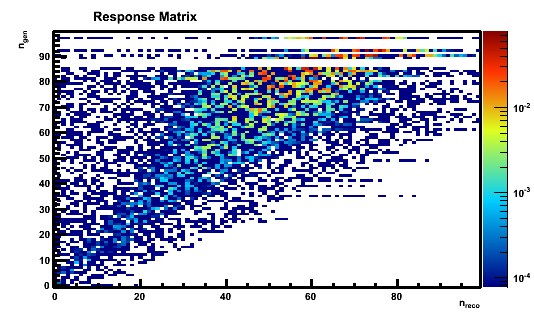
\includegraphics[width=\textwidth]{Chapters/multiplicity/charged_particle_event_multiplicity/images/systematics/response_matrix_diff.png}
		\caption{Difference}
	\end{subfigure}
	\caption{Comparison between the calculated response matrix and the randomised response matrix}
	\label{fig: comparison between calculated response matrix and randomised response matrix}
\end{figure}

\begin{figure}[h]
	\begin{subfigure}{0.49\textwidth}
		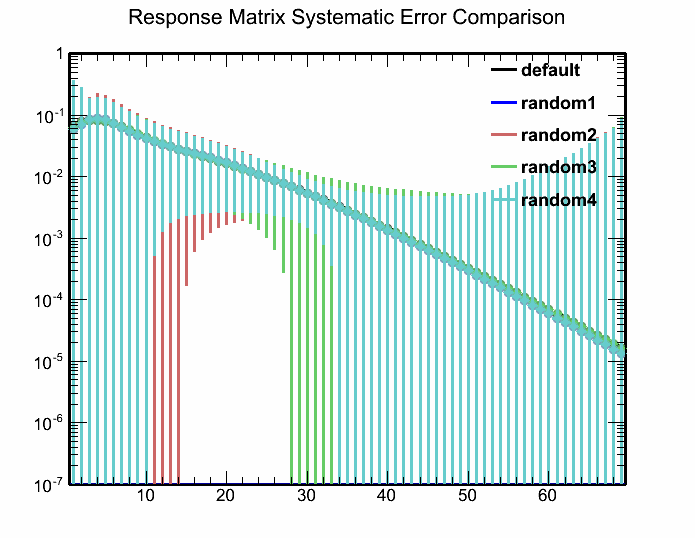
\includegraphics[width=\textwidth]{Chapters/multiplicity/charged_particle_event_multiplicity/images/systematics/random_response_matrix_overlay.png}
		\caption{Comparison of unfolded multiplicities between the default response matrix and the randomised response matrices}
		\label{fig: comparison random response matrices}
	\end{subfigure}
	\begin{subfigure}{0.49\textwidth}
		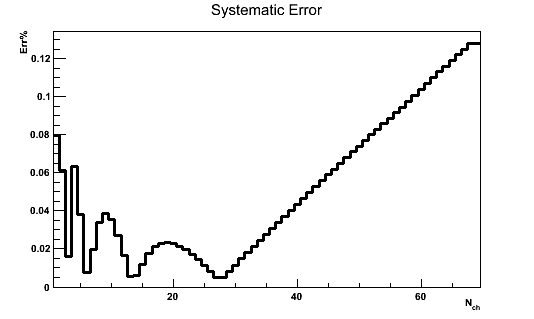
\includegraphics[width=\textwidth]{Chapters/multiplicity/charged_particle_event_multiplicity/images/systematics/random_response_matrix_systematic.png}
		\caption{Response matrix systematic error as a percentage}
		\label{fig: response matrix systematic}
	\end{subfigure}
	\caption{Response matrix systematic errors.}
	\label{fig: response matrix systematic errors}
\end{figure}

In addition to this a systematic uncertainty is due to the parameterisation model used is also present. To estimate this one of the parameterisation models is nominated as the reference parameterisation and the difference between it and the unfolded distributions from the other parameterisations is used to assign an error, figure \ref{fig: parameterisation comparison} shows the comparison between the unfolded distributions due to the different parameterisations and figure \ref{fig: parameterisation systematic} shows the systematic error as a function of the number of charged particles.

\begin{figure}[h]
	\begin{subfigure}{0.49\textwidth}
		\includegraphics[width=\textwidth]{/afs/cern.ch/user/d/dvoong/cmtuser/DaVinci_v33r6/Phys/ChargedParticleMultiplicity/python/multiplicity/tracks/unfolding/systematics/data_files/parameterisations/overlay.png}
		\caption{Comparison of unfolded multiplicities between the default parameterisation and the other parameterisation models}
		\label{fig: parameterisation comparison}
	\end{subfigure}
	\begin{subfigure}{0.49\textwidth}
		\includegraphics[width=\textwidth]{/afs/cern.ch/user/d/dvoong/cmtuser/DaVinci_v33r6/Phys/ChargedParticleMultiplicity/python/multiplicity/tracks/unfolding/systematics/data_files/parameterisations/systematic_error.png}
		\caption{Parameterisation model systematic error as a percentage}
		\label{fig: parameterisation systematic}
	\end{subfigure}
	\caption{Parameterisation model systematic errors.}
	\label{fig: parameterisation model systematic errors}
\end{figure}

The uncertainty in the background correction discussed in section \ref{subsection: charged particle density, systematics} is also present in the measurement of the charged particle event multiplicity, similarly a systematic error of 2\% is applied to the final results.

%\subsection*{Matrix Inversion Unfolding}
%In addition to the unfolding procedure discussed in the previous sections another technique that involves inverting the response matrix was investigated.  The matrix inversion technique involves manipulating equation \ref{equation: multiplicity-response relationship} to give,
%
%\begin{equation}
%	b = R^{-1} \cdot a
%\end{equation}
%
%where $R^{-1}$ is the inverse of the response matrix, $b$ is the true distribution and $a$ is the observed track multiplicity. Inverting the matrix is achieved using Singular Value Decomposition (SVD \cite{wolf:svd}), a numerical method which deconstructs a matrix into a product of two orthogonal matrices and a diagonal matrix. 
%
%\begin{equation}
%	R = u \cdot W \cdot v^\mathrm{T}
%\end{equation}
%
%Hence by using the matrix identities of orthogonal and diagonal matrices,
%
%\begin{equation}
%	u \cdot u^\mathrm{T} = I
%\end{equation}
%
%for orthogonal matices, and
%
%\begin{equation}
%	W^{-1} \cdot W = I
%\end{equation}
%
%by applying matrix multiplication from the left hand side the matrix equation may be written as,
%
%\begin{equation}
%	b = v  \cdot W^{-1} \cdot u^\mathrm{T}
%\end{equation}
%
%In this form the elements of $W^{-1}$ are simply the reciprocals of the diagonal matrix $W$, this leads to vary large elements in $W^{-1}$ which when applied to the orthogonal matrices $u^\mathrm{T}$ and $v$ results in data points with poor statistical significance being amplified (resulting in non-physical results, see figure \ref{fig: unfolded multiplicities matrix inversion}) and the amplification of the oscillatory nature of the orthogonal functions.
%
%\begin{figure}[h]
%	\begin{subfigure}{0.49\textwidth}
%		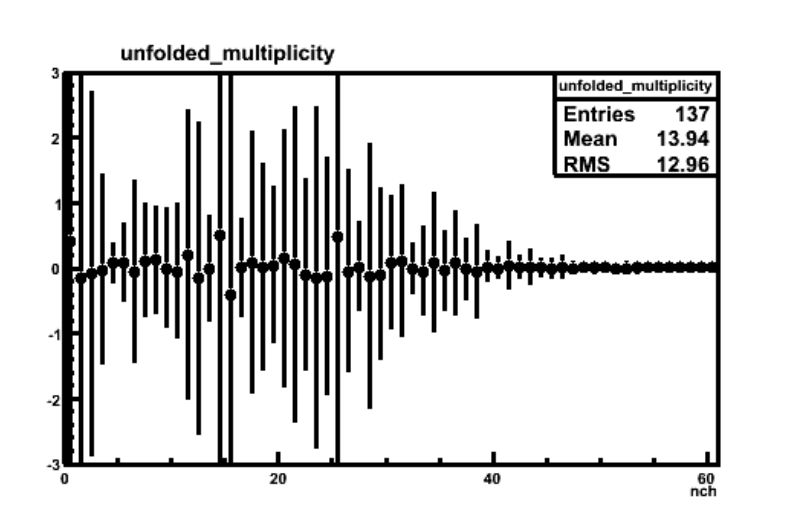
\includegraphics[width=\textwidth]{Chapters/multiplicity/charged_particle_event_multiplicity/images/matrix_inversion/unfolded_multiplicity_mc.png}
%		\caption{MC data}
%	\end{subfigure}
%	\begin{subfigure}{0.49\textwidth}
%		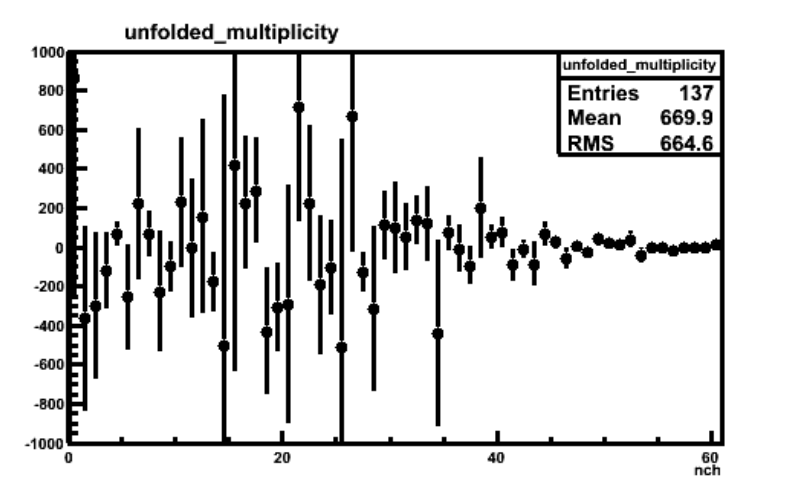
\includegraphics[width=\textwidth]{Chapters/multiplicity/charged_particle_event_multiplicity/images/matrix_inversion/unfolded_multiplicity_real.png}
%		\caption{Real data}
%	\end{subfigure}
%	\caption{Unfolded multiplicities using the matrix inversion method}
%	\label{fig: unfolded multiplicities matrix inversion}
%\end{figure}
%
%By removing contributions of the large weights in $W^{-1}$ (regularising the matrix) these effects may be reduced. 

\subsection*{MC Generator Comparison}

The unfolded multiplicity distribution together with systematic errors is compared with the multiplicity distributions from the Pythia 6, Pythia8 and EPOS event generators in figure \ref{fig: unfolded multiplicity generator comparison}, the average multiplicity for the respective distributions are shown in table \ref{table: multiplicity averages}. The Pythia and EPOS generators show a systematic decrease and increase in higher multiplicity events respectively (in agreement with the charged particle densities).

\begin{table}
	\centering
	\caption{Comparison of the mean charged particle multiplicity between the unfolded multiplicity and MC simulated data}
	\label{table: multiplicity averages}
	\newpage
\begin{table}[h]
	\caption{True multiplicity parameterisations fit to generated prompt particle distributions}
	\label{table: gen multiplicity parameters}
	\begin{subtable}{0.49\textwidth}
		\caption{Parameterisation A}
		\centering
		\begin{tabular}{|c|c|}
			\centering
			p0 & $14.414 \pm 0.988$ \\
			p1 & $-0.19995 \pm 0.181$ \\
			p2 & $17.887 \pm 0.989$ \\
			p3 & $-0.60499 \pm 0.832$ \\
			p4 & $0.01735 \pm 0.332$ \\
			p5 & $1.5373 \pm 0.998$ \\
			p6 & $1.3577 \pm 1.0$ \\
		\end{tabular}
	\end{subtable}
	\begin{subtable}{0.49\textwidth}
		\caption{Parameterisation B}
		\centering
		\begin{tabular}{|c|c|}
			\centering
			p0 & $-4.4678 \pm 33.9$ \\
			p1 & $-0.66946 \pm 2.78$ \\
			p2 & $-2.7404 \pm 53.7$ \\
			p3 & $-1.0328 \pm 11.9$ \\
			p4 & $-6.0631 \pm 33.0$ \\
			p5 & $-0.19869 \pm 0.323$ \\
		\end{tabular}
	\end{subtable}
%	\begin{subtable}{0.49\textwidth}
%		\caption{Parameterisation C}
%		\centering
%		\begin{tabular}{|c|c|}
%			\centering
%			p0 & $1.1237 \pm 3.91$ \\
%			p1 & $0.090301 \pm 0.76$ \\
%			p2 & $23.184 \pm 6.7e+02$ \\
%			p3 & $0.84887 \pm 0.618$ \\
%			p4 & $4.2472 \pm 43.1$ \\
%			p5 & $0.12728 \pm 0.628$ \\
%			p6 & $0.20308 \pm 0.662$ \\
%			p7 & $-0.10058 \pm 1.45$ \\
%		\end{tabular}
%	\end{subtable}
	\begin{subtable}{0.49\textwidth}
		\caption{Parameterisation D}
		\centering
		\begin{tabular}{|c|c|}
			\centering
			p0 & $-17.893 \pm 1.0$ \\
			p1 & $-0.33501 \pm 0.198$ \\
			p2 & $4.1461 \pm 1.04$ \\
			p3 & $-9.5155 \pm 0.993$ \\
			p4 & $-0.22568 \pm 0.178$ \\
			p5 & $3.1305 \pm 0.962$ \\
			p6 & $-2.5895 \pm 0.994$ \\
			p7 & $-0.37285 \pm 0.531$ \\
			p8 & $1.1071 \pm 0.97$ \\
		\end{tabular}
	\end{subtable}
%	\begin{subtable}{0.49\textwidth}
%		\caption{Parameterisation E}
%		\centering
%		\begin{tabular}{|c|c|}
%			\centering
%			p0 & $-6.9649 \pm 11.9$ \\
%			p1 & $-0.1352 \pm 0.302$ \\
%			p2 & $1.074 \pm 0.559$ \\
%			p3 & $16.049 \pm 11.8$ \\
%			p4 & $-0.39655 \pm 0.912$ \\
%			p5 & $-9.7608 \pm 6.69$ \\
%			p6 & $-0.066749 \pm 0.0762$ \\
%			p7 & $7.3009e-05 \pm 0.000732$ \\
%			p8 & $-101.39 \pm 6.09e+04$ \\
%			p9 & $-837.68 \pm 4.06e+04$ \\
%		\end{tabular}
%	\end{subtable}
	\begin{subtable}{0.49\textwidth}
		\caption{Parameterisation F}
		\centering
		\begin{tabular}{|c|c|}
			\centering
			p0 & $-6.3713 \pm 33.5$ \\
			p1 & $-0.20009 \pm 0.272$ \\
			p2 & $-2.6787 \pm 33.5$ \\
			p3 & $-0.6491 \pm 1.08$ \\
		\end{tabular}
	\end{subtable}
\end{table}
\newpage
\end{table}

\begin{figure}[h]
	\includegraphics[width=\textwidth]{/afs/cern.ch/user/d/dvoong/cmtuser/DaVinci_v33r6/Phys/ChargedParticleMultiplicity/python/multiplicity/tracks/data_files/manual/results/canvas.png}
	\caption{The unfolded event multiplicity distribution compared with the Pythia6, Pythia8 and EPOS event generators. The unfolded distribution is shown in black with the systematics shown in the red shaded boxes.}
	\label{fig: unfolded multiplicity generator comparison}
\end{figure}

%\begin{itemize}
%	\item Statistical error: Observed multiplicity propagated to the unfolded multiplicity by the fit to the response/smearing function
%	\item Systematic: Background correction. Main contribution from MC simulation of the detector response to ghost tracks. Also contributions from secondary tracks, tracks from material interaction and a small contribution from clone tracks
%	\item Systematic: Reconstruction efficiency - Statistical uncertainty in the response matrix due to MC statistics
%	\item Systematic: Reconstruction efficiency - How well does MC model the detector efficiency?
%	\item Systematic: Pile up: Not sure how to check?
%	\item Systematic: Events not triggered on - Use MC to check. Systematic from... Can't use data method to estimate
%\end{itemize}

% Unfolded multiplicities with statistical errors
%\begin{figure}[h]
%	\centering
%	\begin{subfigure}{0.49\textwidth}
%		\includegraphics[width=\textwidth]{}
%		\caption{}
%		\label{}
%	\end{subfigure}
%\end{figure}